Описание выбранных методов, моделей, алгоритмов решения задач.

\subsection{ Аппаратная база }
Аппаратная база представлена в виде РВ-90. Это реле на основе микроконтроллера со встроенным Wi-Fi. Аппаратное обеспечение РВ-90 базируется на микроконтроллере RTL8711AM (Realtek, Hsinchu, Тайвань). Характеристиками данного аппаратного обеспечения являются его низкая стоимость, 2 МБ флеш-памяти, встроенная антенна Wi-Fi и чип DS1307 (Maxim Integrated, San Jose, California) для предоставления функций Real time clock (RTC). РВ-90 использует чип RTC в качестве входного сигнала и задает состояние двух выходящих реле как функцию от входного сигнала времени


\subsubsection{ Ядро ARM Cortex-M3 }
Новое семейство процессоров на смену ARM7, призванное занять новую для ARM нишу встраиваемых решений низкой производительности. В семействе присутствуют три значимых ядра.
Cortex-M0 с архитектурой ARMv6-M;
Cortex-M3 (опционально Memory Protection Unit) с архитектурой ARMv7-M;
Cortex-M4 (опционально Floating Point Unit) с архитектурой ARMv7E-M;

\subsubsection{ Микроконтроллер RTL8711AM }
Производства компании Realtek[7], это одно-кристальный микропроцессор нацеленный для изделий для Internet of Things. Он сочетает в себе ARM ядро на базе Cortex-M3, WLAN MAC и NFC в одном чипе. Он также предоставляет 19 GPIO. Конфигурация встроенной памяти RTL8711AM позволяет упростить и ускорить разработку приложений. Есть встроенная RAM и ROM. Выигрывает по характеристикам у более известного ESP8266. Периферия есть на борту. RAM и ROM имеют предопределенную карту памяти. Пользовательский код запускается из Flash память.
\subsubsection{ Модуль RAK473}
Производства компании Rak-Wireless. Интегрируют RTL8711AM с флеш-памятью и антенной на одной печатной плате. У модуля есть документация.  Есть аналогичный модуль компании FN-link F11AMIM13\_B1.
\subsubsection{Реле РВ-90}
Предоставляет светодиоды, исполнительные электромагнитные реле, платы с корпусом и RTC DS1307. Документация на каждую часть. I2C протокол. Типы реле. Выходы и их конфигурация.


\subsection{ Архитектура программы }
В результате проведенного исследования было принято решение о трехкомпонентной архитектуре. Первым компонентом является прошивка, устанавливаемая на РВ-90. Второй компонент представляет собой одно-страничное веб-приложение, которое будет храниться во флеш-памяти вместе с прошивкой.  Третий компонент - это Android-приложение, которое должно быть установлено на устройстве пользователя[12]. Каждый компонент создается с использованием своего стека технологий. Таким образом, программа состоит из трех отдельных компонентов, которые должны быть разработаны отдельно и должны будут взаимодействовать друг с другом. 

Конструкция аппаратной базы для РВ-90 является фиксированной и должна учитываться при проектировании архитектуры программы

\textbf{Три платформы}
\begin{my_itemize}
\item РВ-90
\item Браузер
\item Android
\end{my_itemize}


\begin{figure}[h!]
    \centering
    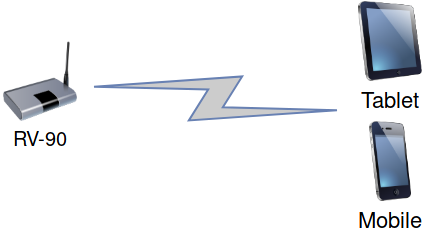
\includegraphics[width=0.7\textwidth]{three_platforms.png}
    \caption{Рисунок 3. Диаграмма взаимодействия между реле и клиентом.}
\end{figure}



\subsubsection{ Проектирование архитектуры прошивки для РВ-90 }
Что должна делать прошивка.
Безопасность и надежность являются первостепенными задачами. На основе анализа соответствующей работы был разработан ряд руководящих принципов и решений. Во-первых, сеть Wi-Fi должна быть размещена самим РВ-90 (рис. 3). Это поможет снизить риск безопасности, связанный с распространением информации через Интернет. Во-вторых, прошивка будет написана на языке программирования Rust. Это ограничит количество ошибок связанных с переполнением буфера, стека и ряда других типичных для приложений написанных на языке C. Использование Rust также должно упростить тестирование, поскольку юнит- тесты являются частью языка, что будет способствовать поддержанию качество кода. Ожидается, что безопасность будет дополнительно повышена путем выбора руководящих принципов MISRA-C, которые могут применяться в контексте языка программирования Rust. 

Использование SoC на основе ARM означает, что Rust может использоваться в качестве языка программирования для выбора прошивки вместо C. необходимо также учитывать тот факт, что флеш-память ограничена 2 МБ. Часть этого пространства должна быть зарезервирована для прошивки, часть для веб-приложения и часть для пользовательских данных. Веб-приложение должно быть как можно меньше, чтобы поместиться во флеш-память вместе с изображениями, шрифтами, библиотеками и другими необходимыми данными. Программа для контроля и мониторинга РВ-90 должна создавать и поддерживать собственную сеть WiFi, чтобы устройство работало даже в зоне без подключения к интернету. Таймер RTC DS1307 имеет разрешение точности до миллисекунды, для того чтобы удовлетворить требованиям для точного времени.

Прошивка устанавливается на РВ-90 в процессе производства.  Прошивка разбивается на несколько модулей. Модули разделены на основе функциональности, которая должна присутствовать в реле времени. Устройство каждого из модулей.

\begin{my_itemize}
\item Модуль управления многозадачностью и аппаратным разделением ресурсов.
\item Модуль для управления выходом реле (включено-выключено).
\item Модуль для работы стека TCP/IP и управления сетью Wi-Fi.
\item Модуль вывода отладочной информации.
\item Модуль управления HTTP сервером.
\item Модуль для анализа и генерации ответа на запросы API.
\item Модуль для анализа и генерации JSON.
\item Модуль для управления коммуникацией по протоколу I2C.
\item Модуль для связи с чипом DS1307 в режиме реального времени.
\item Модуль управления временем системы.
\item Модуль управления файловой системой.
\end{my_itemize}

\subsubsection{ Проектирование архитектуры веб-интерфейса}
Что должен делать каждый из модулей.

Веб-приложение будет написано в Typescript, чтобы свести к минимуму вероятность ошибок во время выполнения.

Пользовательский интерфейс реализован в веб-приложении. Оно предоставляет тот же функционал который можно встретить в других электронных реле времени. Оператор может: создать новый цикл включения/выключения и дать ему имя, назначить цикл определенному дню и установить его на повторение еженедельно или ежемесячно, установить исключения и переопределить циклы в определенные дни, получить обзор того, какие циклы выполняются в какие дни. Интерфейс интуитивно понятен и прост в использовании.

Одно-страничное веб-приложение хранится во флеш-памяти РВ-90 вместе с прошивкой. При подключении оно передается на телефон или планшет пользователя через браузер и в нем же и запускается. Веб-приложение можно разложить на следующие модули:

\begin{my_itemize}
\item Модуль для взаимодействия с сервером через AJAX.
\item Модуль для отображения состояния реле.
\item Модуль для настройки цикла включения / выключения на один день.
\item Модуль для настройки дней выполнения для цикла включения/выключения.
\item Модуль для отображения циклов включения/выключения и календарь циклов.
\item Модуль, чтобы помочь пользователю с началом работы.
\item Модуль для отображения ошибок и информационных сообщений.
\end{my_itemize}



\subsubsection{Проектирование архитектуры приложения Android}
На смартфоне установлено приложение для Android. Он используется для подключения к РВ-90, загрузки веб-приложения и запуска его. Он должен содержать следующие модули:

\begin{my_itemize}
\item Модуль для управления учетными данными Wi-Fi.
\item Модуль для подключения к сети Wi-Fi РВ-90.
\item Модуль для запроса, получения, запуска и остановки веб-приложения.
\end{my_itemize}


\subsection{Выводы по главе}
Рассмотрены архитектуры трех компонент программы. Спроектировано их взаимодействие, а также их взаимодействие с пользователем, спроектирована общая архитектура программы.

